\section{Informationsdarstellung}
\subsection{Begriffe}
\todo{Woche2: Word abhängig von Verarbeitungsbreite.}

\subsection{Signale}
\todo{Woche2: Signale, Daten-Meldungen, Datenströme}

\subsection{Zahlendarstellung}
\todo{TODO}
\subsubsection{Vorzeichenlose Ganzzahl}
\[W = \sum_{i=0}^{n-1}d_i\cdot 2^i\]
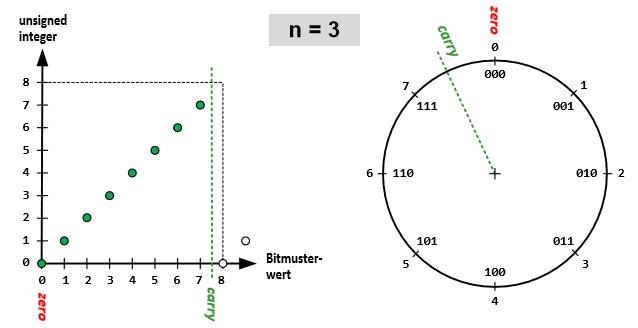
\includegraphics[width=\linewidth]{Images/ganzzahl}


\subsubsection{Signed Magnitued}
\[W = (-1)^{n-1} \cdot \sum_{i=0}^{n-1}d_i\cdot 2^i\]
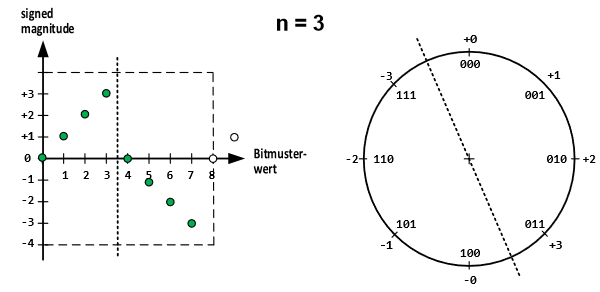
\includegraphics[width=\linewidth]{Images/signedmagnetude}

\subsubsection{Einerkomplement}
\[
W =
\begin{cases}
	\sum_{i=0}^{n-2}d_i \cdot 2^i & d_{n-1} > 0 \\
	\left(\sum_{i=0}^{n-2}d_i \cdot 2^i\right) - \sum_{i=0}^{n-2}2^i & d_{n-1} < 0 
\end{cases}
\]
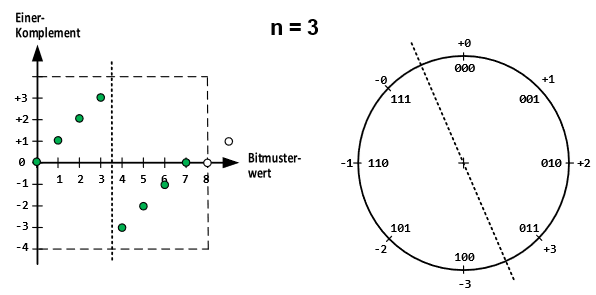
\includegraphics[width=\linewidth]{Images/einerkomplement}


\subsubsection{Zweierkomplement}
\[W = \left(\sum_{i=0}^{n-1}d_i\cdot 2^i\right) - (d^{n-1}\cdot2^n)\]
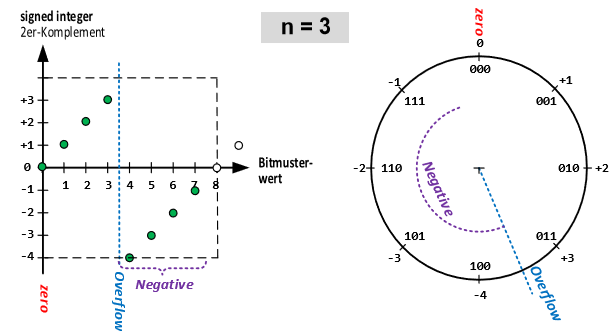
\includegraphics[width=\linewidth]{Images/zweierkomplement}

\subsubsection{Excess-Code (EX)}
\[W = \left(\sum_{i=0}^{n-1}d_i\cdot 2^i\right) - (2^{n-1})\]
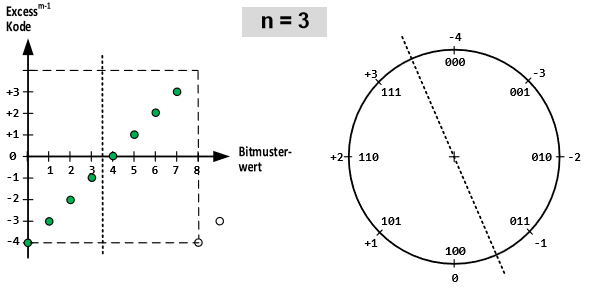
\includegraphics[width=\linewidth]{Images/ex}


\subsubsection{Festkommazahl}
\todo{Basisformat, Fraktionale Zahlen, IQ-Zahlen}

\subsubsection{Gleitkommazahl}
Binär zu Dezimal IEEE 754\\
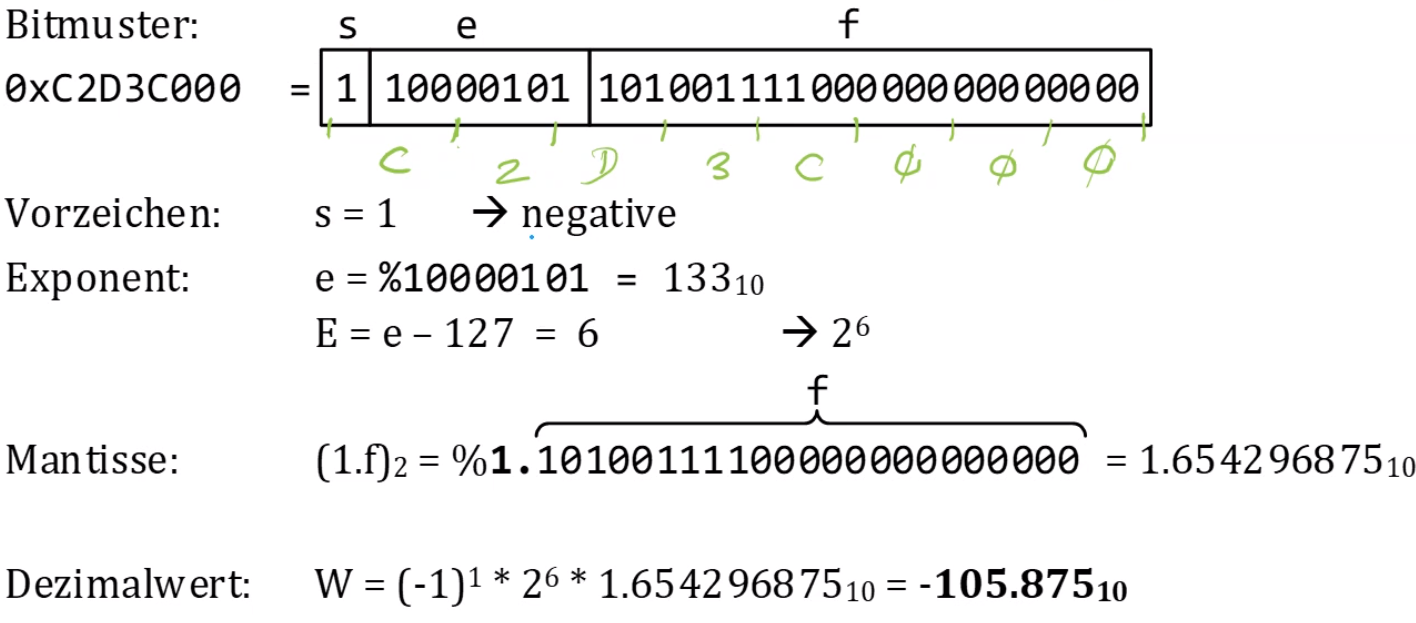
\includegraphics[width=\linewidth]{Images/float}

\subsubsection{BCD-Code}